
\titledquestion{Making Binary Trees Grow}


\begin{parts}

    %%%%%%%%%%%%%%%%%%%%%%%%%%%%%%%%%%%%%%%%%%%%%%%%%%%%%%%%%%
    % (a) Inorder + Preorder: 3 points
    %%%%%%%%%%%%%%%%%%%%%%%%%%%%%%%%%%%%%%%%%%%%%%%%%%%%%%%%%%

    \part[3]
    Given the \textbf{inorder} and \textbf{preorder}
    traversals of a binary tree $T$ shown below,
    draw the tree $T$.

    \begin{center}
    \begin{tabular}{ll}
        \textbf{Inorder:}  & $\mathbf{CFHKMPWXY}$ \\
        \textbf{Preorder:} & $\mathbf{PHCFMKWYX}$
    \end{tabular}
    \end{center}

    \begin{solutionorbox}

        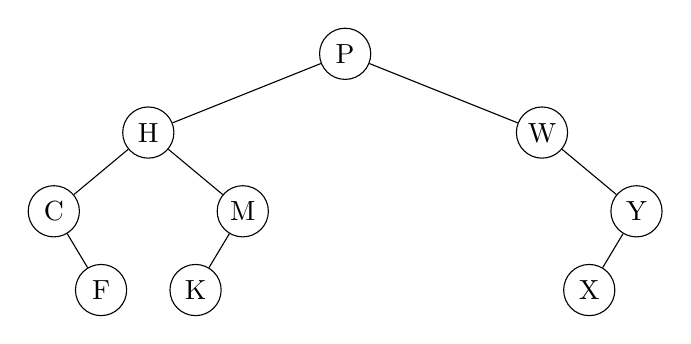
\begin{tikzpicture}[
        every node/.style={circle, draw, minimum size=0.65cm, inner sep=0pt}
        ]
        \node (P) at (0, 0)     {P};

        \node (H) at (-2.5, -1) {H};
        \node (W) at (2.5, -1)  {W};

        \node (C) at (-3.7, -2) {C};
        \node (M) at (-1.3, -2) {M};
        \node (Y) at (3.7, -2)  {Y};

        \node (F) at (-3.1, -3) {F};
        \node (K) at (-1.9, -3) {K};
        \node (X) at (3.1, -3)  {X};

        \draw (P) -- (H);
        \draw (P) -- (W);

        \draw (H) -- (C);
        \draw (H) -- (M);

        \draw (C) -- (F);
        \draw (M) -- (K);

        \draw (W) -- (Y);
        \draw (Y) -- (X);
        \end{tikzpicture}
    \end{solutionorbox}


    %%%%%%%%%%%%%%%%%%%%%%%%%%%%%%%%%%%%%%%%%%%%%%%%%%%%%%%%%%
    % (b) Inorder + Postorder: 3 points
    %%%%%%%%%%%%%%%%%%%%%%%%%%%%%%%%%%%%%%%%%%%%%%%%%%%%%%%%%%

    \part[3]
    Given the \textbf{inorder} and \textbf{postorder}
    traversals of a binary tree $T$ shown below,
    draw the tree $T$.

    \begin{center}
    \begin{tabular}{ll}
        \textbf{Inorder:}   & $\mathbf{BCDRQNTVWYZ}$ \\
        \textbf{Postorder:} & $\mathbf{CBDNQTWZYVR}$
    \end{tabular}
    \end{center}

    \begin{solutionorbox}
        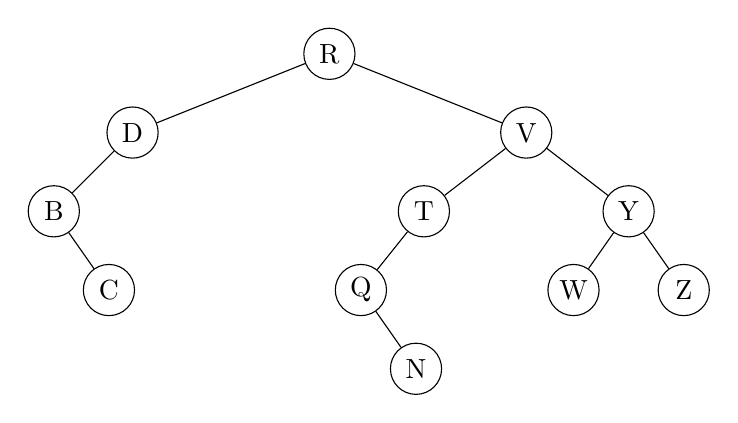
\begin{tikzpicture}[
        every node/.style={circle, draw, minimum size=0.65cm, inner sep=0pt}
        ]
        % 1. 节点位置定义 (x, y)
        \node (R) at (0, 0)     {R};

        \node (D) at (-2.5, -1) {D};
        \node (V) at (2.5, -1)  {V};

        \node (B) at (-3.5, -2) {B};
        \node (T) at (1.2, -2)  {T};
        \node (Y) at (3.8, -2)  {Y};

        \node (C) at (-2.8, -3) {C};
        \node (Q) at (0.4, -3)  {Q};
        \node (W) at (3.1, -3)  {W};
        \node (Z) at (4.5, -3)  {Z};

        \node (N) at (1.1, -4)  {N};

        % 2. 边的连接
        \draw (R) -- (D);
        \draw (R) -- (V);

        \draw (D) -- (B);

        \draw (B) -- (C);

        \draw (V) -- (T);
        \draw (V) -- (Y);

        \draw (T) -- (Q);

        \draw (Q) -- (N);

        \draw (Y) -- (W);
        \draw (Y) -- (Z);
        \end{tikzpicture}
    \end{solutionorbox}


    %%%%%%%%%%%%%%%%%%%%%%%%%%%%%%%%%%%%%%%%%%%%%%%%%%%%%%%%%%
    % (c) Preorder + Postorder: 2 points
    %%%%%%%%%%%%%%%%%%%%%%%%%%%%%%%%%%%%%%%%%%%%%%%%%%%%%%%%%%

    \part[2]
    Do the \textbf{preorder} and \textbf{postorder}
    traversal sequences uniquely determine an arbitrary
    binary tree $T$? If yes, briefly explain how to reconstruct it.
    If no, draw \textbf{two different binary trees}, each with
    at least four nodes, that have the same preorder and
    postorder traversal sequences.

    \begin{solutionorbox}
        No.

        Assuming a binary tree with only a root and a leaf. No matter where the leaf is, the preorder traversal is always `root-leaf, and the postorder traversal is always `leaf-root`. Therefore, the preorder and postorder traversal sequences do not uniquely determine an arbitrary binary tree.

        Example:

        \begin{tikzpicture}[
        every node/.style={circle, draw, minimum size=0.65cm, inner sep=0pt}
        ]
        \node (A1) at (0, 0)  {A};
        \node (B1) at (-0.8, -1) {B};
        \node (C1) at (-1.6, -2) {C};
        \node (D1) at (-2.4, -3) {D};

        \draw (A1) -- (B1);
        \draw (B1) -- (C1);
        \draw (C1) -- (D1);

        \node[draw=none] at (-1.2, -4) {\textbf{Tree 1}};

        \node (A2) at (4, 0)   {A};
        \node (B2) at (4.8, -1) {B};
        \node (C2) at (5.6, -2) {C};
        \node (D2) at (6.4, -3) {D};

        \draw (A2) -- (B2);
        \draw (B2) -- (C2);
        \draw (C2) -- (D2);

        \node[draw=none] at (5.2, -4) {\textbf{Tree 2}};
        \end{tikzpicture}
    \end{solutionorbox}

\end{parts}
